\section*{Обработка результатов измерений}

1. Рассчитаем для каждой пары значений тока $ I $ и напряжения $ U_e $
значения $ P, P_e, \eta, \dfrac{R_1}{R_i} = \dfrac{U_e}{(E - U_e)} $ для $ G_1 $.
\\
\\

$ G_1, E_1 = 7.4 $ В

\begin{tabular}{|c|c|c|c|c|c|c|}
    \hline
    i & $ U_e $, В & $ I(U_e) $, А & $ P = E*I $, Вт & $ P_e = U_e*I $, Вт & $ \eta = \dfrac{P_e}{P} $ & $ \dfrac{R_1}{R_i} = \dfrac{U_e}{(E - U_e)} $\\
    \hline
    1 & $ 0 $ & $ 0.0082 $ & $ 0.0607 $ & $ 0.0 $ & $ 0.0 $ & $ 0.0 $\\
    \hline
    2 & $ 1 $ & $ 0.007 $ & $ 0.0518 $ & $ 0.007 $ & $ 0.1351 $ & $ 0.1562 $\\
    \hline
    3 & $ 2 $ & $ 0.006 $ & $ 0.0444 $ & $ 0.012 $ & $ 0.2703 $ & $ 0.3704 $\\
    \hline
    4 & $ 3 $ & $ 0.005 $ & $ 0.037 $ & $ 0.015 $ & $ 0.4054 $ & $ 0.6818 $\\
    \hline
    5 & $ 4 $ & $ 0.0038 $ & $ 0.0281 $ & $ 0.0152 $ & $ 0.5409 $ & $ 1.1765 $\\
    \hline
    6 & $ 5 $ & $ 0.0027 $ & $ 0.02 $ & $ 0.0135 $ & $ 0.675 $ & $ 2.0833 $\\
    \hline
\end{tabular}\\
\\
\\

2. Рассчитаем для каждой пары значений тока $ I $ и напряжения $ U_e $
значения $ P, P_e, \eta, \dfrac{R_1}{R_i} = \dfrac{U_e}{(E - U_e)} $ для $ G_2 $.
\\
\\

$ G_2, E_2 = 6.2 $ В

\begin{tabular}{|c|c|c|c|c|c|c|}
    \hline
    i & $ U_e $, В & $ I(U_e) $, А & $ P = E*I $, Вт & $ P_e = U_e*I $, Вт & $ \eta = \dfrac{P_e}{P} $ & $ \dfrac{R_1}{R_i} = \dfrac{U_e}{(E - U_e)} $\\
    \hline
    1 & $ 0 $ & $ 0.0094 $ & $ 0.0583 $ & $ 0.0 $ & $ 0.0 $ & $ 0.0 $\\
    \hline
    2 & $ 1 $ & $ 0.0079 $ & $ 0.049 $ & $ 0.0079 $ & $ 0.1612 $ & $ 0.1923 $\\
    \hline
    3 & $ 2 $ & $ 0.0064 $ & $ 0.0397 $ & $ 0.0128 $ & $ 0.3224 $ & $ 0.4762 $\\
    \hline
    4 & $ 3 $ & $ 0.0049 $ & $ 0.0304 $ & $ 0.0147 $ & $ 0.4836 $ & $ 0.9375 $\\
    \hline
    5 & $ 4 $ & $ 0.0032 $ & $ 0.0198 $ & $ 0.0128 $ & $ 0.6465 $ & $ 1.8182 $\\
    \hline
    6 & $ 5 $ & $ 0.0019 $ & $ 0.0118 $ & $ 0.0095 $ & $ 0.8051 $ & $ 4.1667 $\\
    \hline
\end{tabular}
\\
\\

\newpage

3. Построим на одном рисунке для каждого источника зависимости 
$ P, P_e, \eta $ от отношения $ \dfrac{R_1}{R_i} $ для $ G1 $.

\begin{figure}[hpt!]
    \centering
    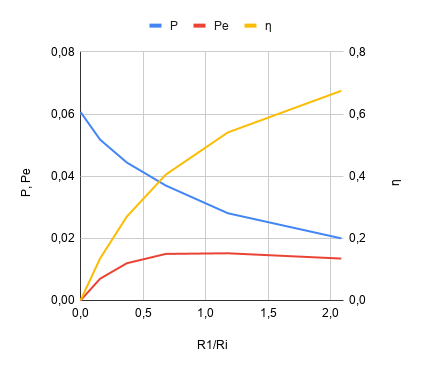
\includegraphics[width=0.6\linewidth]{photo/chart_g1}
\end{figure}

4. Построим на одном рисунке для каждого источника зависимости 
$ P, P_e, \eta $ от отношения $ \dfrac{R_1}{R_i} $ для $ G2 $.

\begin{figure}[hpt!]
    \centering
    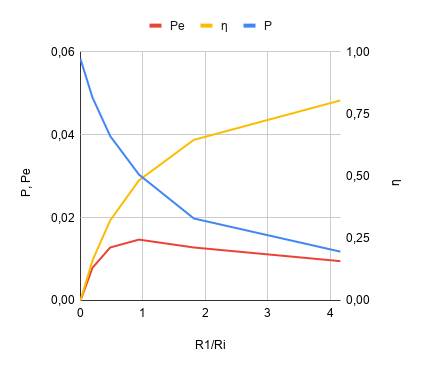
\includegraphics[width=0.6\linewidth]{photo/chart_g2}
\end{figure}

\newpage

5. Определим для $ G_1 $:
$ P_{e max}, P_{K3} $, внутреннее сопротивление $ R_i $.\\

$ R_i = \dfrac{E - U_e}{I} $\\

$ G_1, E_1 = 7.4 $ В

\begin{tabular}{|c|c|c|c|}
    \hline
    i & $ U_e $, В & $ I(U_e) $, А & $ R_i = \dfrac{E - U_e}{I} $\\
    \hline
    1 & $ 0 $ & $ 0.0082 $ & $ 902.44 $\\
    \hline
    2 & $ 1 $ & $ 0.007 $ & $ 914.29 $\\
    \hline
    3 & $ 2 $ & $ 0.006 $ & $ 900.0 $\\
    \hline
    4 & $ 3 $ & $ 0.005 $ & $ 880.0 $\\
    \hline
    5 & $ 4 $ & $ 0.0038 $ & $ 894.74 $\\
    \hline
    6 & $ 5 $ & $ 0.0027 $ & $ 888.89 $\\
    \hline
\end{tabular}
\\
\\

$ \overline R_i = 
\dfrac{\sum R_{i i}}{N} = 
\dfrac{5380.36}{6} = 
896.72
$ Ом
\\

$ P_{e\ max} = 
\dfrac{E^2}{4R_i} = 
\dfrac{54.76}{4 * 896.72} = 
0.01526674993308948
$ Вт
\\

$ P_{K3} = 
\dfrac{E^2}{R_i} = 
P_{e\ max} * 4 = 
0.06106699973235792
$ Вт
\\

6. Определим для $ G_2 $:
$ P_{e max}, P_{K3} $, внутреннее сопротивление $ R_i $.\\

$ G_1, E_2 = 6.2 $ В

\begin{tabular}{|c|c|c|c|}
    \hline
    i & $ U_e $, В & $ I(U_e) $, А & $ R_i = \dfrac{E - U_e}{I} $\\
    \hline
    1 & $ 0 $ & $ 0.0094 $ & $ 659.57 $\\
    \hline
    2 & $ 1 $ & $ 0.0079 $ & $ 658.23 $\\
    \hline
    3 & $ 2 $ & $ 0.0064 $ & $ 656.25 $\\
    \hline
    4 & $ 3 $ & $ 0.0049 $ & $ 653.06 $\\
    \hline
    5 & $ 4 $ & $ 0.0032 $ & $ 687.5 $\\
    \hline
    6 & $ 5 $ & $ 0.0019 $ & $ 631.58 $\\
    \hline
\end{tabular}
\\
\\

$ \overline R_i = 
\dfrac{\sum R_{i i}}{N} = 
\dfrac{3946.19}{6} = 
657.7
$ Ом
\\

$ P_{e\ max} = 
\dfrac{E^2}{4R_i} = 
\dfrac{38,44}{4 * 657.7} = 
0.014611562038320508
$ Вт
\\

$ P_{K3} = 
\dfrac{E^2}{R_i} = 
P_{e\ max} * 4 = 
0.05844624815328203
$ Вт
\\
